\documentclass[11pt,mathserif]{beamer}
\usepackage[utf8]{inputenc}
\usepackage[english]{babel}
\usepackage{tikz}
\usepackage{amsmath,amssymb,mathtools,dsfont}
\usepackage{tensortyping}
%\usepackage{movie15}
\usepackage{multimedia}
%\usepackage[]{biblatex}

\usepackage{pgfplots}
\usepgfplotslibrary{patchplots}
\usepgfplotslibrary{groupplots}
\pgfplotsset{compat=1.3}

\newcommand{\roughcite}[1]{\textit{#1}}

\usetheme[titlepagelogo=Avancez_black.pdf,notitleflower]{chalmers}

% Some some front page information
\title{Multiscale Modeling of Sintering of Hardmetal}
%\subtitle{And something more}
\author{Mikael Öhman}
\institute{Dept. of Applied Mechanics\\ Chalmers University of Technology}
\date{NSCM23, KTH, Stockholm, November 22--23 2010}
% Bibliography
%\bibliography{references_extended}

\begin{document}

\section{Title page}
\begin{frame}[plain]
 \titlepage
\end{frame}

\section{Outline}
\begin{frame}
 \frametitle{Outline}

\begin{itemize}
 \item Background --- Motivation
 %\item Surface tension
 %\item Sintering phenomena on mesoscale
 \item Remarks on constitutive modeling
 \item Multiscale modeling
 \item FE-code OOFEM: Object Oriented Finite Element Method
 \item Conclusions --- Future work
\end{itemize}
\end{frame}

\section{Background}
% \begin{frame}
%  \frametitle{Project background and motivation}
%  \begin{itemize}
%   \item Complicated macroscopic constitutive models
%   \begin{itemize}
%     \item Many parameters, impossible to measure
%     \item Needs experimental calibration
%   \end{itemize}
%   \item Computational power increasing
%  \end{itemize}
% 
%  \roughcite{Mähler, Ekh \& Runesson (1999)}
% 
%  \roughcite{Svoboda \& Reidel  (1996)}
% \end{frame}

\subsection{Process}
\begin{frame}
 \frametitle{Background --- Sintering of hardmetal}

% The sintering phenomenon on the mesoscale is driven by surface tension on the melted binder, and
% the homogenized effect of the surface tension is the so-called sintering stress.
% From the macroscopic perspective, the specimen (green body) shrinks due to this volumetric sintering stress. In the case of inhomogeneous
% initial density in the green body, the sintering can result in unwanted final deformations.

 \begin{enumerate}
  %\item Mixture of WC and Co particles (micrometer size)
  \item WC-particles surrounded by Co-matrix (binder metal)
  %\item Heating and softening of binder
  \item Precompaction $\rightarrow$ initial porosity 20--40\%
  \item Heating $\rightarrow$ thermal expansion, sintering driven by surface tension in Co-porespace
  \item Vanishing final porosity (ideal state)
  
  %\item Melting binder

  %\item Bridging between particles
  %\item Particles aggregate
  %\item Compaction due to surface tension
 \end{enumerate}
\alert{Note: Inhomogeneous initial density may lead to defect product:\\ \textsuperscript{(i)}remaining porosity, \textsuperscript{(ii)}shape imperfection }
\begin{center}
 \begin{columns}
 \column{0.25\textwidth}\centering
 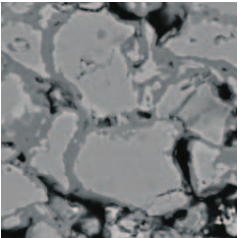
\includegraphics[width=\textwidth]{figures/sinter_1-crop.pdf}
 \column{0.05\textwidth}\centering
 $\xrightarrow{\text{idealized}}$
 \column{0.25\textwidth}\centering
 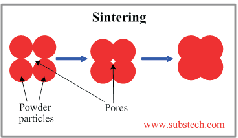
\includegraphics[width=\textwidth]{figures/sinter_2-crop.pdf}
  
 \end{columns}

 %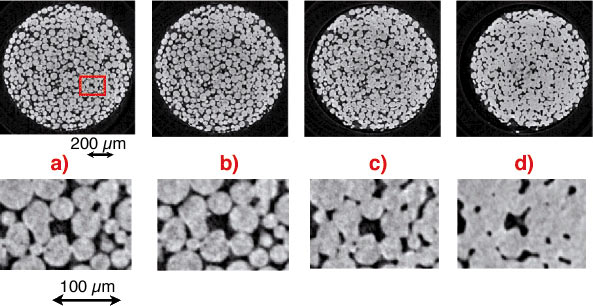
\includegraphics[width=0.6\textwidth]{figures/fig081.jpeg}
\end{center}
\end{frame}

\subsection{Comparison}
\begin{frame}
 \frametitle{Constitutive modeling}
 Macroscopic modeling
 \begin{itemize}
  \item Selected references: \roughcite{Svoboda \& Riedel (1996)}, \roughcite{Mähler, Ekh \& Runesson (1999)}
  \item Complex model structure, requires many parameters --- calibration problem very ill-posed
 \end{itemize}

 Multiscale modeling
 \begin{itemize}
  \item Selected references:  \roughcite{Geers \& coworkers (2001--)},
 \roughcite{Fish \& coworkers (1995--)},
 \roughcite{Miehe \& coworkers (2002--)},
 \roughcite{Larsson \& Runesson [adaptive multiscale] (2006--)}
  \item Modeling of \textsuperscript{(i)}solid WC, \textsuperscript{(ii)}melt Co and \textsuperscript{(iii)}surface tension\\
  Note: Constitutive modeling refers to subscale constituents
  \item FE$^2$ (FE on macro and mesoscales) based on computational homogenization on RVE:s
  \item Macroscale: Momentum balance
 \end{itemize}
\end{frame}

\section{Mesoscale}
\begin{frame}
 \frametitle{Mesoscale modeling of sintering}

 \begin{itemize}
  \item Incompressible nonlinear Stokes flow problem
  \item Finite element
  \begin{itemize}
    \item Taylor-Hood element (quadratic $\to v$, linear $p$)
    \item Surface tension element
  \end{itemize}
  \item Explicit time stepping
  \item Updated Lagrangian formulation
  %\item Simple constitutive driver
  \item \alert{Note: Finite macroscale compressibility despite incompressible subscale flow}
 \end{itemize}

\begin{figure}[hbpt]
 \centering
%  \begin{tikzpicture}
%   \begin{groupplot}[
%     group style={group size=3 by 1},
%     width=4cm,
%     height=4cm,
%     xticklabels={},
%     yticklabels={},
%     %colormap/cool,
%     patch to triangles,
%     %patch refines=1,
% 	%shader=interp,
% 	%shader=flat,
%     %colorbar style={y=Pressure,title=Colorbar},
%    point meta min={-1.6}, % Had to look them manually. Might be possible to fetch from the first plot though.
%    point meta max={1.16}
%    ]
%   \nextgroupplot
%   \addplot[patch,patch table={figures/connectivity_tri2.dat},patch type=triangle quadr, ultra thin, point meta=\thisrow{p}]
%     table[x=x,y=y] {figures/nodes_1.dat};
%   \addplot[patch,mesh,patch table={figures/connectivity_edge.dat},patch type=quadratic spline, thick, draw=black]
%     table[x=x,y=y] {figures/nodes_1.dat};
%   \nextgroupplot%[xtick=\emtpy]
%   \addplot[patch,patch table={figures/connectivity_tri2.dat},patch type=triangle quadr, ultra thin, point meta=\thisrow{p}]
%     table[x=x,y=y] {figures/nodes_50.dat};
%   \addplot[patch,mesh,patch table={figures/connectivity_edge.dat},patch type=quadratic spline, thick, draw=black]
%     table[x=x,y=y] {figures/nodes_50.dat};
%   \nextgroupplot%[colorbar,colorbar right, colorbar style={ylabel=Pressure}]
%   \addplot[patch,patch table={figures/connectivity_tri2.dat},patch type=triangle quadr, ultra thin, point meta=\thisrow{p}]
%     table[x=x,y=y] {figures/nodes_200.dat};
%   \addplot[patch,mesh,patch table={figures/connectivity_edge.dat},patch type=quadratic spline, thick, draw=black]
%     table[x=x,y=y] {figures/nodes_200.dat};
%   \end{groupplot}
%   \draw[thick,black,->,shorten >=5pt,shorten <=5pt] (group c1r1.east) -- (group c2r1.west);
%   \draw[thick,black,->,shorten >=5pt,shorten <=5pt] (group c2r1.east) -- (group c3r1.west);
%  \end{tikzpicture}
 \caption{Evolution of free surface within an RVE}\label{fig:rve_evolution}
\end{figure}
\end{frame}

\newcommand{\macroscale}{\mathrm{M}}
\newcommand{\subscale}{\mathrm{s}}
\begin{frame}
 \frametitle{RVE--problem: Viscous sintering}
 \begin{center}
  \begin{columns}
   \column{0.2\textwidth}
   \column{0.3\textwidth}\centering
    \resizebox{!}{0.8\textwidth}{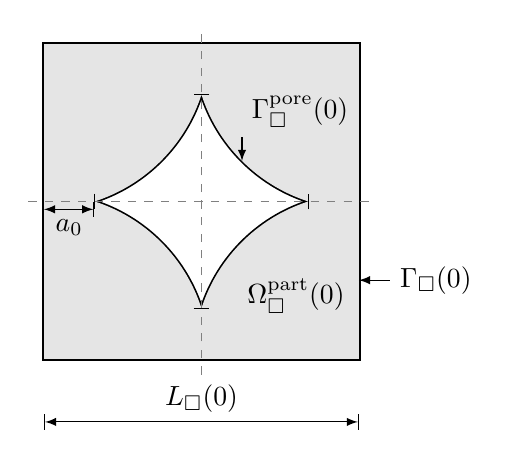
\begin{tikzpicture}[>=latex,scale=2] % Use this to scale the image. Text is always normal-size
  \def\particleradius{1.05} % Adjust this to change the contact size.
  \pgfmathsetmacro{\contactsize}{sqrt(\particleradius^2-1)} % Automatically calculated.
  \begin{scope}[very thick]
  	\draw[clip] (-1,-1) rectangle (1,1);
  	\draw[clip]
  		(-1,-1) circle (\particleradius)
 		( 1,-1) circle (\particleradius)
 		(-1, 1) circle (\particleradius)
   		( 1, 1) circle (\particleradius);
  	\fill[fill=black!10] (-1,-1) rectangle (1,1);
  \end{scope}
  % Markers
  \foreach \q in {0,90,180,270} { \draw[rotate=\q] (1-\contactsize,-0.05) -- +(0,0.1); }
  \draw[dashed,gray] (-1.1,0) -- (1.1,0) (0,-1.1) -- (0,1.1);
  % Annotations
  %\node[below] at (0,0) {$\Omega_\Box^p(0)$};
  \draw[|<->|] (-1,-1.4) -- (1,-1.4) node[midway,above] {$L_\Box(0)$};
  \draw[<->|] (-1,-0.05) -- +(\contactsize,0) node[midway,below] {$a_0$};
  \node at (0.6,-0.6) {$\Omega_\Box^{\mathrm{part}}(0)$};
  \draw[<-] (1,-0.5) -- +(0.2,0) node[right] {$\Gamma_\Box(0)$};
  \draw[<-] (1,1) ++(-135:\particleradius) -- +(0.00,0.15) node[above right] {$\Gamma_\Box^{\mathrm{pore}}(0)$};
  
  %\draw[use as bounding box] (-1.7,-1.5) rectangle (1.7,1.1);
  %\useasboundingbox (-1.7,-1.5) (1.7,1.1);
  % Transformation arrow (makes the picture very unaligned)
  %\draw[->] (1.5,0) to[out=45,in=-150] (2,0);% +(135:0.1) -- (2,0) -- +(-135:0.1);
\end{tikzpicture}
}
   \column{0.3\textwidth}\centering
    \resizebox{!}{0.8\textwidth}{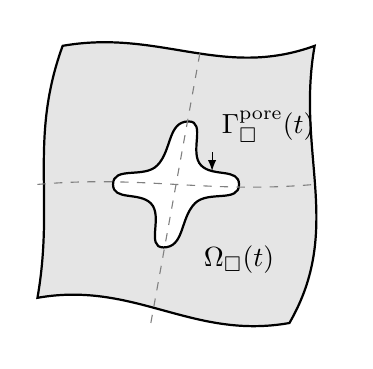
\begin{tikzpicture}[>=latex,scale=1.6] % Use this to scale the image. Text is always normal-size
  \def\particleradius{1.05} % Adjust this to change the contact size.
  \draw[thick,fill=black!10,even odd rule] (0.9,-1.1) 
  	to[out=190,in=10] (-1.1,-0.9)
  	to[out=80,in=-110] (-0.9,1.1)
  	to[out=10,in=-160] (1.1,1.1)
  	to[out=-100,in=60] (0.9,-1.1) -- cycle
  	(-0.1,-0.5) to[out=180,in=-45] (-0.2,-0.15) to[out=135,in=-90]
  	(-0.5,0)    to[out=90,in=-135] (-0.15,0.15)  to[out=45,in=-180]  
  	(0.1,0.5)   to[out=0,in=135]   (0.2,0.15)   to[out=-45,in=90] coordinate[near start] (GammaF)
  	(0.5,0)     to[out=-90,in=45]  (0.15,-0.15)  to[out=-135,in=0] (-0.1,-0.5) -- cycle;
  % Markers
  \draw[dashed,gray] (-1.1,0) to[out=5,in=-175] (1.1,0) (-0.2,-1.1) -- (0.2,1.1);
  % Annotations
  \node at (0.5,-0.6) {$\Omega_\Box(t)$};
  \draw[<-] (GammaF) -- +(0.00,0.15) node[above right] {$\Gamma_\Box^{\mathrm{pore}}(t)$};
\end{tikzpicture}}
   \column{0.2\textwidth}
  \end{columns}
 \end{center}
 \begin{itemize}
  \item Suface-tension driven microflow of single unit cell RVE
  \item RVE-problem with Dirichlet b.c. ``driven'' by macroscale rate-of-deformation $\bar{\ts d}\rightarrow$ subscale velocity:
	$\ts v = \ts v^\macroscale(\bar{\ts d})+\ts v^\subscale$

 For given $\bar{\ts d}$, solve for $\ts v^\subscale \in \mathds{V}_\square^{\mathrm{D}}, p \in \mathds{P}_\square$:
 \begin{align*}
  a_\square(\ts v^\macroscale(\bar{\ts d})+\ts v^\subscale; \delta\ts v^\subscale) + b_\square(p,\delta \ts v^\subscale) &= l_\square(\delta \ts v^\subscale)\quad &&\forall \delta \ts v^\subscale \in \mathds{V}_\square^{(\mathrm{D})},\\
 b_\square(\delta p,\ts v^\macroscale(\bar{\ts d}) + \ts v^\subscale) &= 0 && \forall \delta p\in \mathds P_\square.
 \end{align*}

 $l_\square(\delta \ts v^\subscale)$: loading by ``sintering stresses'' = surface tension tractions on $\Gamma_\square^{\text{pore}}$
 \end{itemize}


\end{frame}


\subsection{Surface Tension}
\begin{frame}
 \frametitle{RVE-problem: Modeling of surface tension}
 \begin{itemize}
  \item Traction from curvature of free surfaces
 \begin{gather*}
  \to t = 2\kappa\gamma \to n
\end{gather*}
 \item Weak form (based on surface-divergence theorem)
\begin{gather*}
 \gamma\int_\Omega 2 \kappa \to w\cdot \to n\intd A = \gamma\int_{\partial\Omega} \to w\cdot\to m\intd S - \gamma\int_\Omega \to \nabla_s \cdot \to w \intd A
 \label{eq:curvature}
\end{gather*}
 \roughcite{Steinmann \& Javili (2008--)}
 \item \alert{Note: Geometry dependent!} Possible to compute a tangent for higher order approximation

 \item Difficult/Costly to express load in Backward Euler scheme due to topological changes of merging surfaces

 \roughcite{Perić \& Coworkers (2006)}
 \end{itemize}
\end{frame}

\subsection{Results}
\begin{frame}
 \frametitle{Numerical results: Single RVE}
\begin{center}
\movie[height=6cm,width=6cm,poster]{}{RVE_Fixed_Boundaries.avi}

\movie[externalviewer]{RVE with fixed boundaries --- macroscopically isochoric deformation}{RVE_Fixed_Boundaries.avi}
\end{center}
\end{frame}

\begin{frame}
 \frametitle{Numerical results: Single RVE}
\begin{center}
\movie[height=6cm,width=6cm,poster]{}{RVE_Sheared_Boundaries.avi}

\movie[externalviewer]{RVE with sheared boundaries -- macroscopically rigid}{RVE_Sheared_Boundaries.mpeg}
\end{center}
\end{frame}

\section{Macroscale}
\begin{frame}
 \frametitle{Multiscale implementation}
\begin{columns}
\column{0.51\textwidth}
 Subscale
 \begin{itemize}
  \item Dirichlet b.c. on RVE
 \end{itemize}

 Macroscale
 \begin{itemize}
  \item Large deformations
  %\begin{itemize}
   \item Updated Lagrangian formulation
   %\item Nonlinear
  %\end{itemize}
  \item Compressible up to a certain point
 \end{itemize}

\column{0.49\textwidth}

\begin{center}
 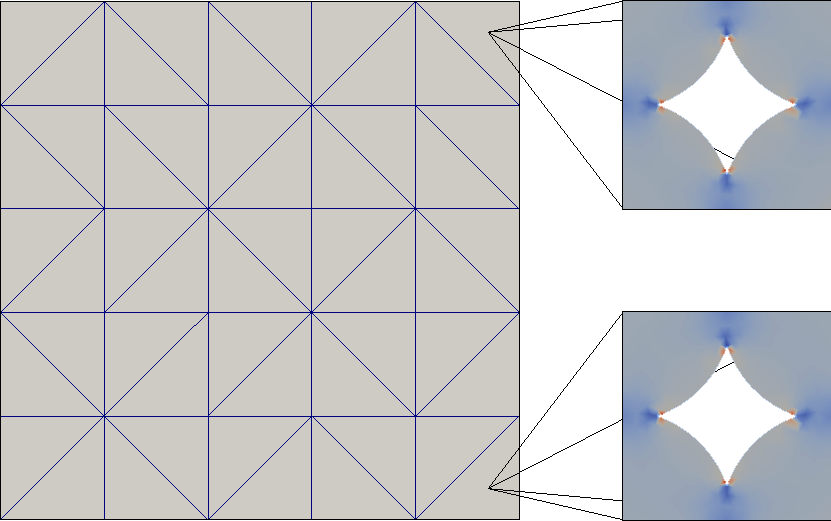
\includegraphics[width=0.9\textwidth]{figures/Sintering_5x5_000.png}\\
 $\longrightarrow$\\[0.5em]
 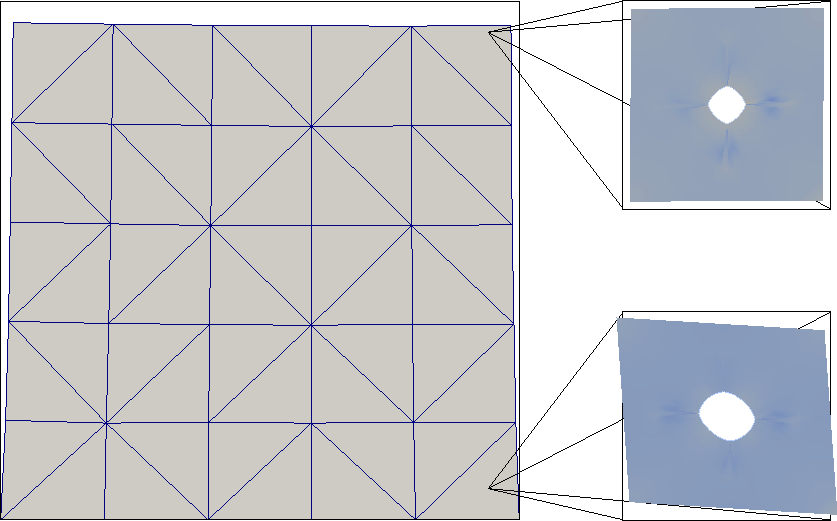
\includegraphics[width=0.9\textwidth]{figures/Sintering_5x5_114.png}
\end{center}
\end{columns}
\end{frame}

\subsection{Results}
\begin{frame}
 \frametitle{Numerical results}
\begin{center}
\movie[height=6cm,width=9.7cm,poster]{}{Sintering_5x5.avi}

\movie[externalviewer]{Multiscale sintering}{Sintering_5x5.mpeg}
\end{center}
\end{frame}

\section{Implementation}
\subsection{OOFEM}
\begin{frame}
 \frametitle{OOFEM -- Finite element code}
 Implementation
 \begin{enumerate}
  \item Implementing constitutive drivers for macroscale
  \item Subscale FE-problem replaces conventional constitutive model
  \item Some difficulties fitting into the design of OOFEM
 \end{enumerate}

\onslide<2-> Some positive notes
 \begin{enumerate}
  \item<2-> Parallel computations: Already designed for message passage paradigm.
  \item<2-> Nonlinear solvers
  \begin{itemize}
   \item<2-> Several linear solvers
   \item<2-> Line-search solvers
   \item<2-> Newton solvers
  \end{itemize}
  \item<2-> Exporting data
  \item<2-> Adaptivity
  \item<2-> Cooperation, \url{http://www.oofem.org/}
 \end{enumerate}

\end{frame}

\section{Future}
\begin{frame}
 \frametitle{Conclusions --- Future work}
 Requirements for realistic microstructures
 \begin{enumerate}
  \item Remeshing
  \begin{itemize}
   \item Levelset representation of voids and particles
   \item Multiple surfaces
   \item Vanishing pores
  \end{itemize}
  \item 3D
 \end{enumerate}
 Other work
 \begin{enumerate}
  \item Weakly periodic boundary conditions (Neumann boundary condition as special case)
  \item Comparison against macroscopic experiments.
 \end{enumerate}

\end{frame}

% \section{End of presentation}
% \begin{frame}
%  \frametitle{Thank you!}
%  \nocite{*}
%  \printbibliography{}
% \end{frame}


\end{document}
